%
% splitting.tex --
%
% (c) 2019 Prof Dr Andreas Mueller, Hochschule Rapperswil
%
\section{Splitting the solution}
\rhead{Splitting the solution}
We would like to better understand the solution space of a linear partial
differential equation of second order with operator $L$.
We start with the formulation
\begin{equation}
\begin{aligned}
Lu&=f&&\qquad\text{in $\Omega$}\\
 u&=g&&\qquad\text{on $\partial\Omega$,}
\end{aligned}
\label{pdgl2ord:allg}
\end{equation}
of the problem and are looking for solutions.
Because the equation is linear, we can attempt to build the solution
as a linear combination of functions that each partially solve the
problem.

In a first step, we try to solve the equation without regard to the
boundary conditions.
We call such a solution a particular solution and denote it $u_p$, it solves
\index{particluar solution}
\begin{equation}
Lu_p=f\qquad\text{in $\Omega$.}
\label{pdgl2ord:up}
\end{equation}
We don't require anything about the values of $u_p$ on the boundary
$\partial\Omega$.

To solve the original problem, we now need an additional summand $u_r$
that takes care of the boundary values.
In order for $u_p+u_r$ to be a better solution of the original problem,
it still has to solve the partial differential equation:
\[
L(u_p+u_r)=f+Lu_r=f\qquad\Rightarrow\qquad Lu_r=0.
\qquad\text{in $\Omega$.}
\]
In addition, we want to make sure that the boundary conditions
\[
u_p+u_r=g\qquad\Rightarrow\qquad u_r=g-u_p\qquad\text{auf $\partial\Omega$}
\]
are satisfied.
So the function $u_r$ has to be a solution of the following partial
differential equation problem:
\begin{equation}
\begin{aligned}
Lu_r&=0&&\qquad\text{in $\Omega$}\\
 u_r&=g-u_p&&\qquad\text{auf $\partial\Omega$}
\end{aligned}
\label{pdgl2ord:ur}
\end{equation}
Note that $u_r$ satisfies a simpler partial differential equation,
simpler mainly because it is homogenous.
The complication has been shifted to the boundary values.

It could still be possible that the original problem has more solutions
than the one just found.
We should be able to find such solutions from $u_p+u_r$ by adding
an additional term $u_h$.
This term must not destroy what we have accomplished with the first
two steps,
it therefore must satisfy the equations
\begin{equation}
\begin{aligned}
L(u_p+u_r+u_h)&=f+Lu_h&&\Rightarrow&Lu_h&=0&&\text{in $\Omega$}\\
  u_p+u_r+u_h &=g +u_h&&\Rightarrow& u_h&=0&&\text{auf $\partial\Omega$}
\end{aligned}
\label{pdgl2ord:uh}
\end{equation}
A solution of the problem~(\ref{pdgl2ord:allg}) thus consists of three
terms $u_p$, $u_r$ and $u_h$:
\begin{enumerate}
\item
$u_p$ solves the differential equation~(\ref{pdgl2ord:up}) disregarding
the boundary conditions.
\item
$u_r$ solves the differential equation~(\ref{pdgl2ord:ur}),
$u_p+u_r$ solves the original problem.
\item
If the homogeneous problem~(\ref{pdgl2ord:uh}) with homogeneous
\index{homogeneous}
boundary conditions has nontrivial solution, then the solution
of the original problem is not unique.
Any solution $u_h$ of the homogeneous problem gives an additional
solution.
\end{enumerate}

\begin{beispiel}
\begin{figure}
\centering
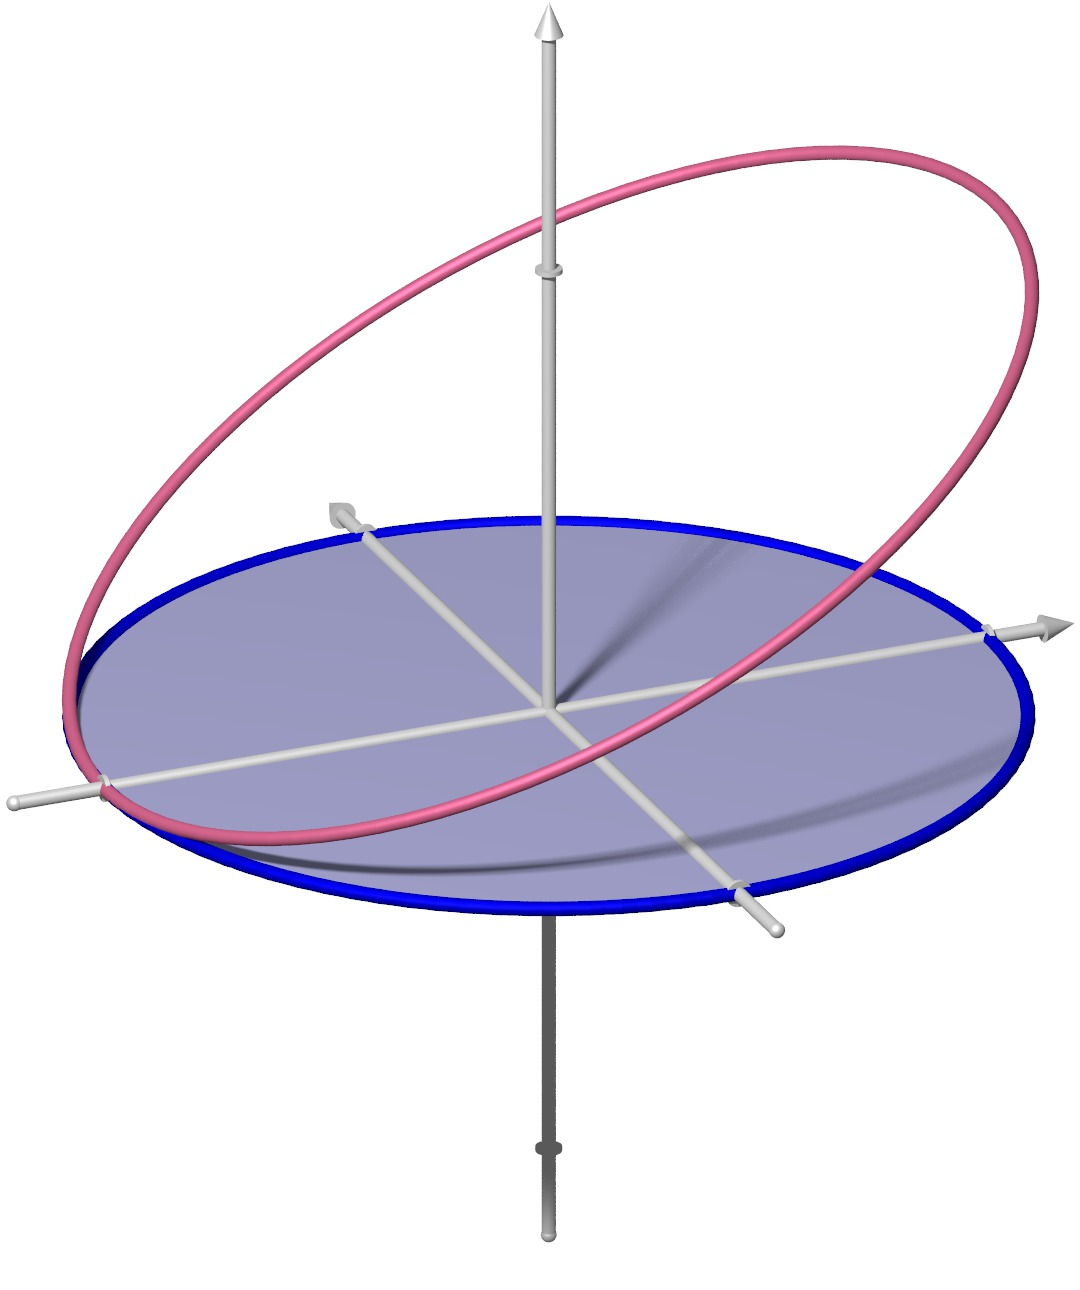
\includegraphics[width=0.44\hsize]{6-2ord/images/problem.jpg}
\qquad
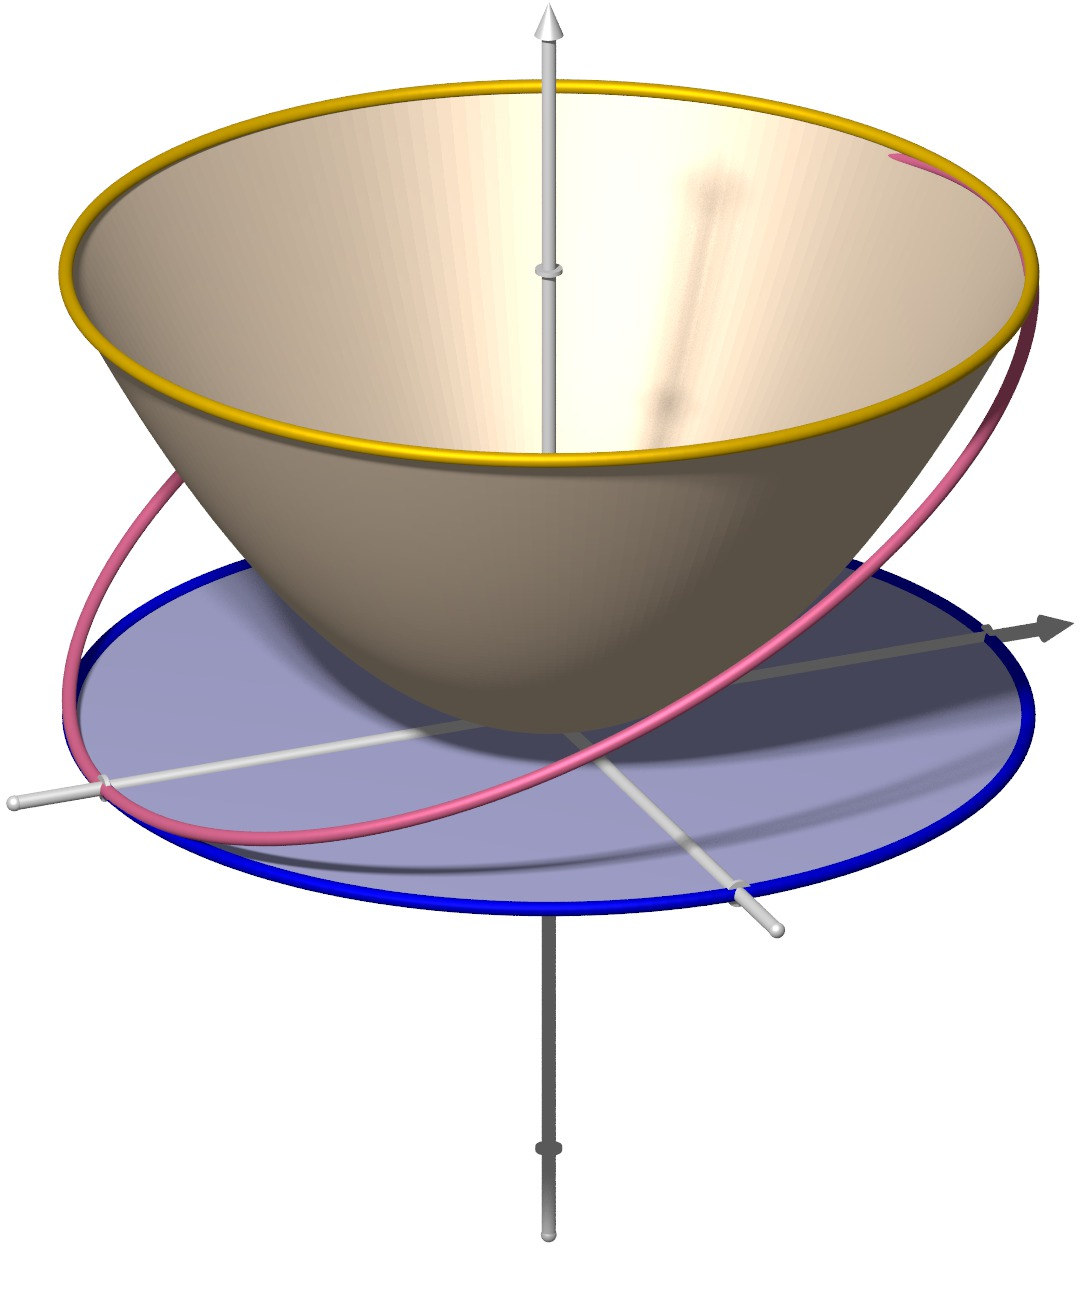
\includegraphics[width=0.44\hsize]{6-2ord/images/particular.jpg}
\caption{Boundary values and domain (left) and particular solution (right)
for the example problem~\eqref{2ord:splitexample}
\label{2ord:splitfigure}}
\end{figure}
\begin{figure}
\centering
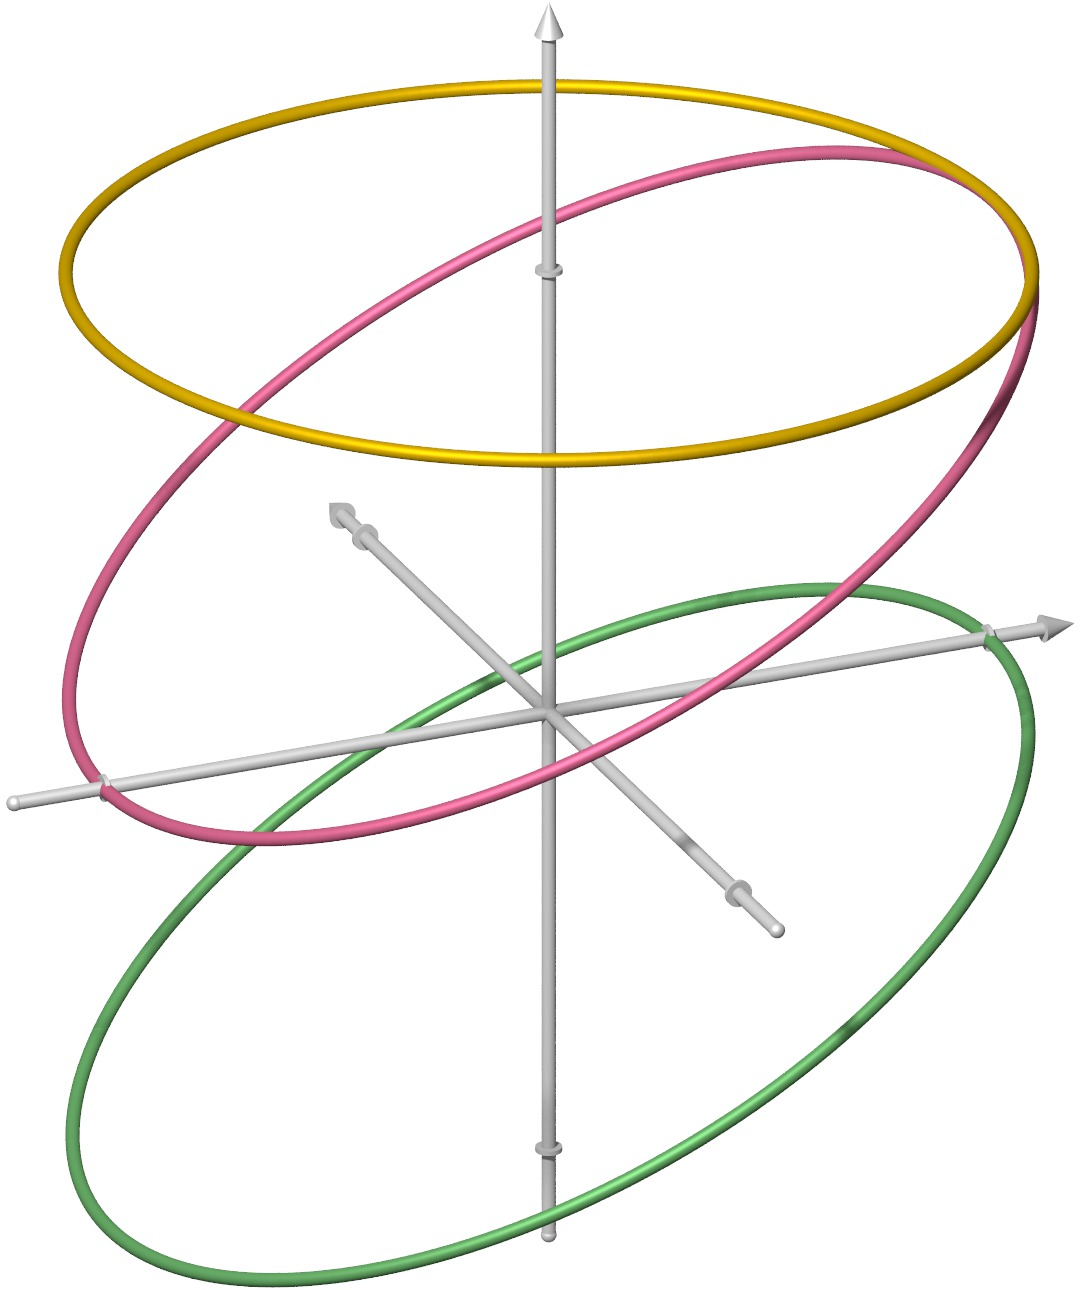
\includegraphics[width=0.44\hsize]{6-2ord/images/rproblem.jpg}
\qquad
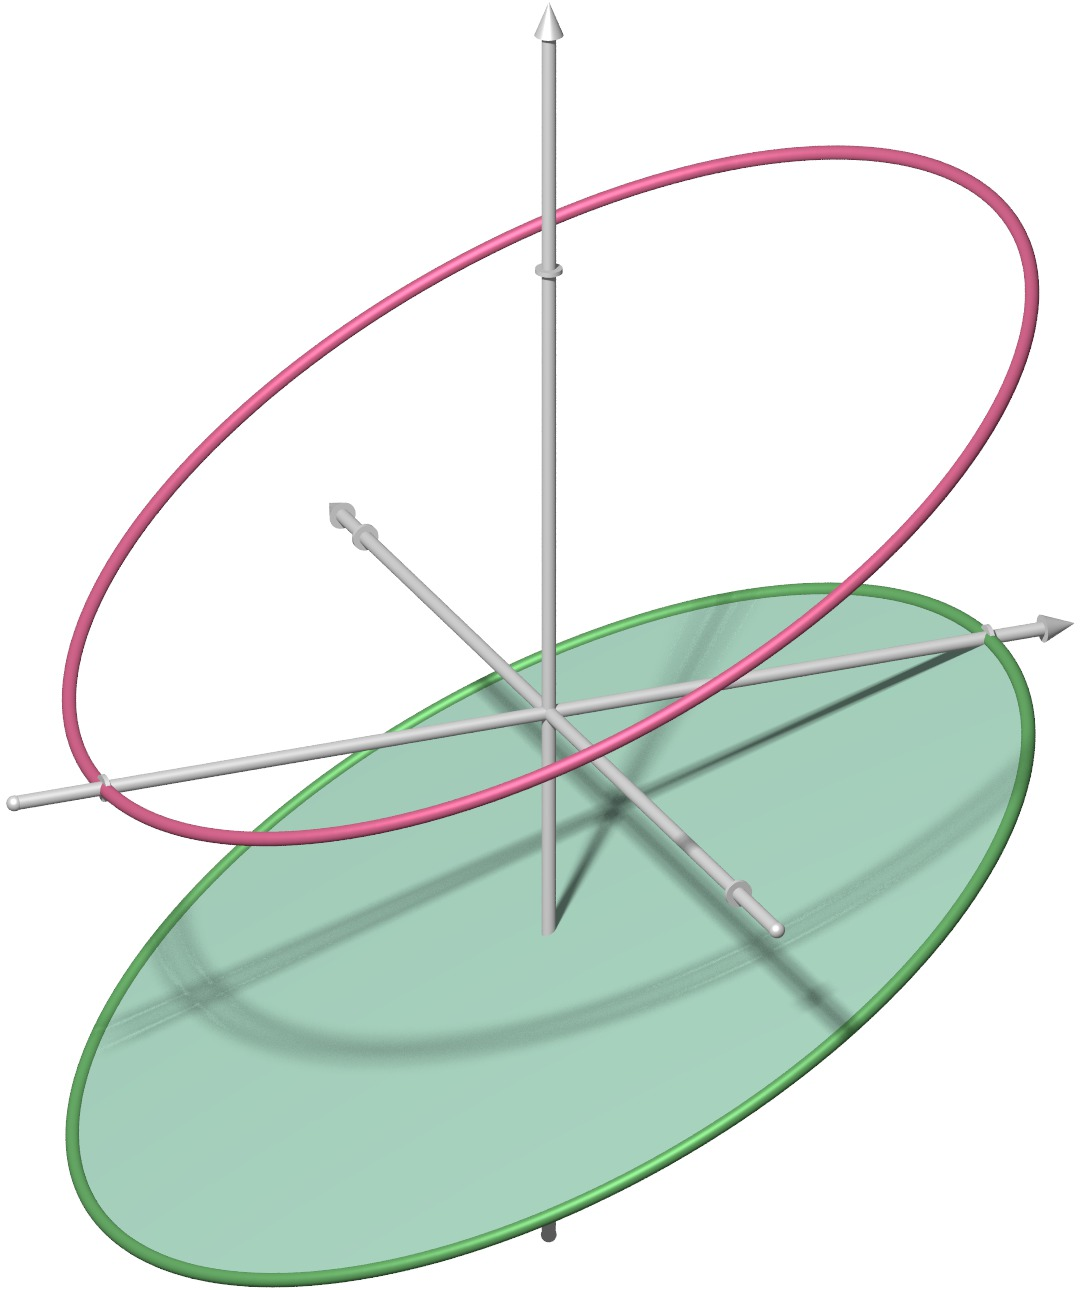
\includegraphics[width=0.44\hsize]{6-2ord/images/rsolution.jpg}
\caption{Boundary values for $u_r$ (left) and solution $u_r$ (right)
for the example problem~\eqref{2ord:splitexample}.
\label{2ord:splitur}}
\end{figure}
\begin{figure}
\centering
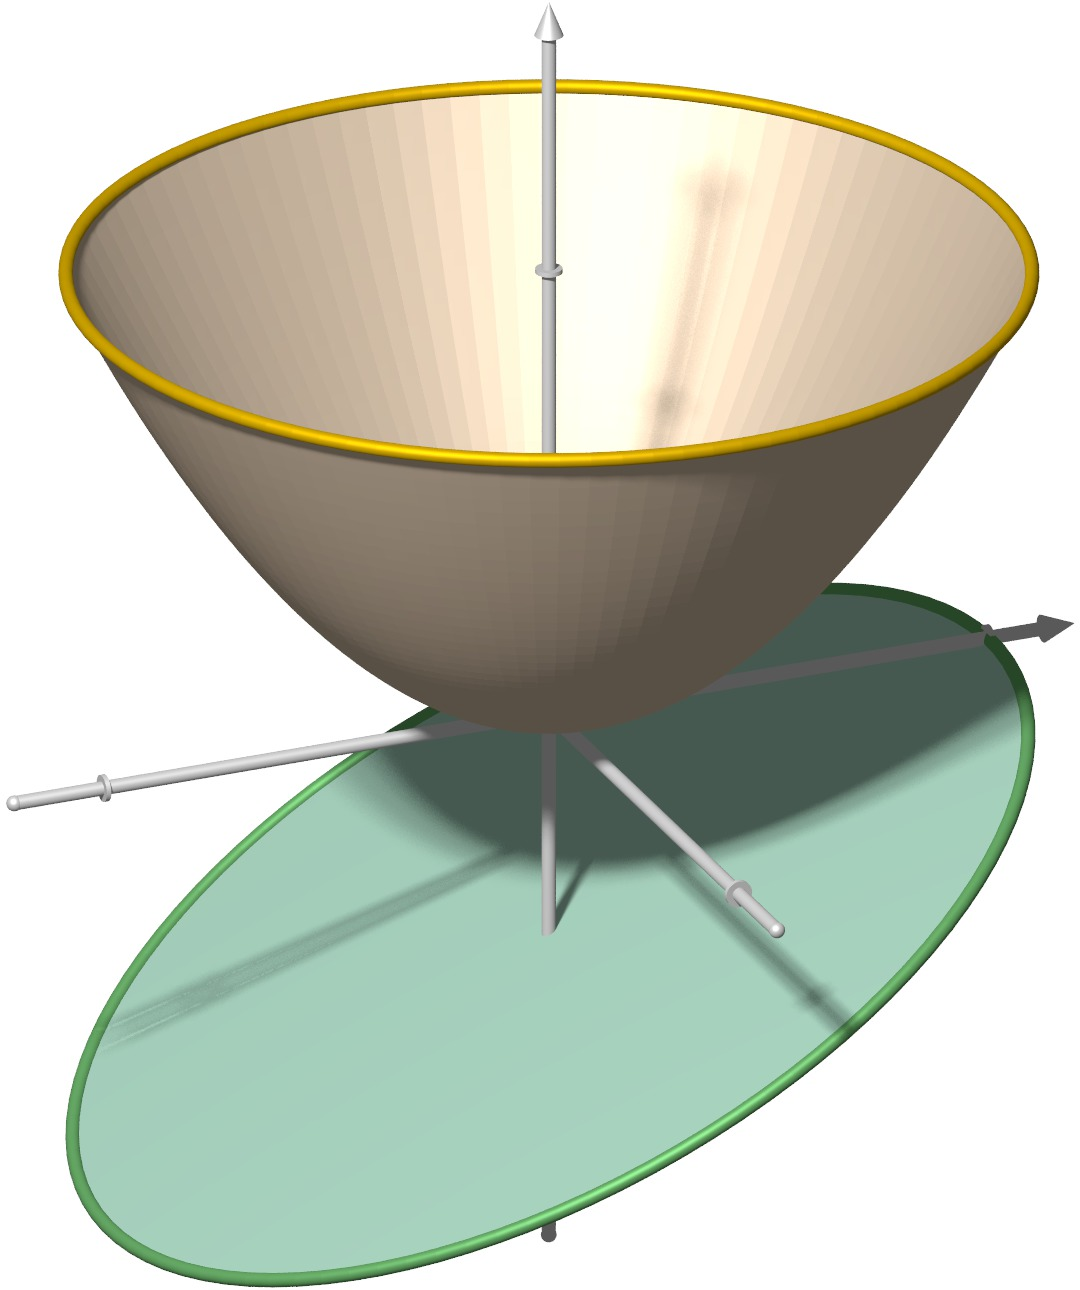
\includegraphics[width=0.44\hsize]{6-2ord/images/combine.jpg}
\qquad
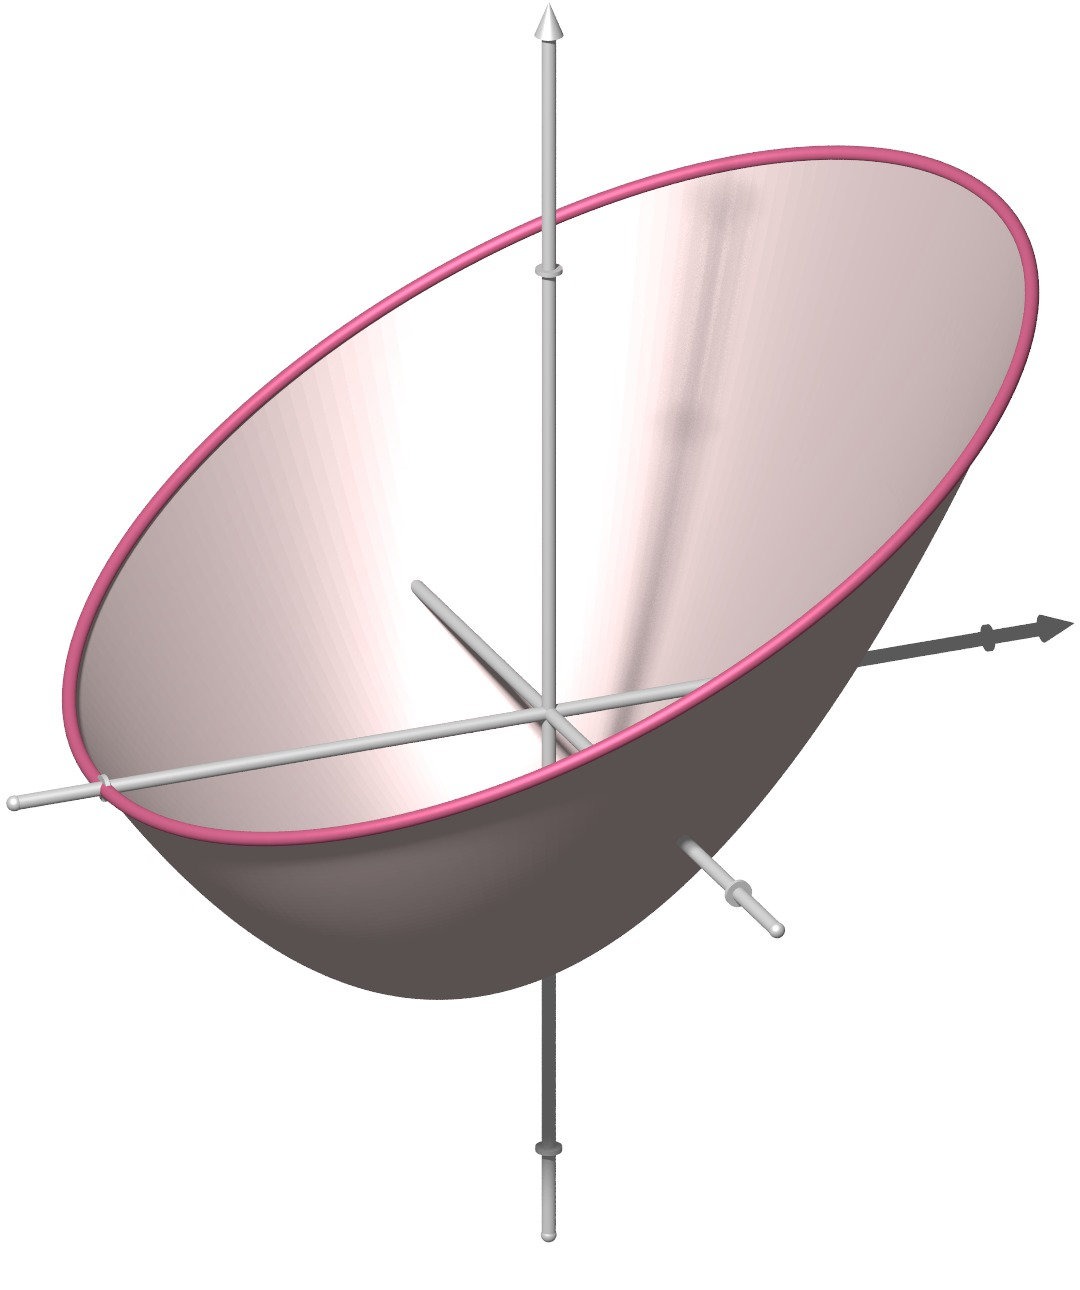
\includegraphics[width=0.44\hsize]{6-2ord/images/solution.jpg}
\caption{$u_p$ and $u_r$ (left) for 
for the example problem~\eqref{2ord:splitexample}
and the combined final solution (right).
\label{2ord:splitsol}}
\end{figure}
Consider the partial differential equation problem on the unit
disk $\Omega=\{(x,y)\,|\,x^2+y^2<1\}$
\begin{align}
\Delta u &= 4
\quad\text{in $\Omega$}
&
u&=\frac12x+\frac12
\quad\text{on $\partial\Omega$}
\label{2ord:splitexample}
\end{align}
This problem data is illustrated in figure~\ref{2ord:splitexample} left.

First we have to find a particular solution.
The function $u_p(x,y)=x^2+y^2$ is such a solution.
The graph of $u_p$ is illustrated in 
figure~\ref{2ord:splitexample} on the right.
Obviously the boundary conditions (pink) are not satisfied.

To fix the boundary conditions, we have to find a solution $u_r$ of the
homogeneous problem with boundary values 
\begin{equation}
u_r
=
\frac12x+\frac12-u_p(x,y)
= 
\frac12x+\frac12-1
=
\frac12x-\frac12.
\label{2ord:ur}
\end{equation}
These boundary values are illustrated as the green curve in 
figure~\ref{2ord:splitur}.
The right hand side of~\eqref{2ord:ur} happens to be a solution
of the homogeneous equation.
The complete solution then is the sum of the two,
\[
u(x,y)
=
u_p(x,y)+u_r(x,y)
=
x^2 + y^2 + \frac12x-\frac12
\]
This is also illustrated in figure~\ref{2ord:splitsol}.
\end{beispiel}

